% various abbreviations
\renewcommand{\L}{{\mathscr{L}}}
\newcommand{\MSbar}{$\overline{\mathrm{MS}}$}
\newcommand{\BR}{{\text{BR}}}
\newcommand{\LO}{{\text{LO}}}
\newcommand{\NLO}{{\text{NLO}}}
\newcommand{\EW}{{\text{EW}}}
\newcommand{\QCD}{{\text{QCD}}}
\newcommand{\QED}{{\text{QED}}}
\newcommand{\LEP}{{\text{LEP}}}
\newcommand{\SLD}{{\text{SLD}}}

\newcommand{\SM}{{\text{SM}}}
\newcommand{\PH}{\text{Higgs}}
\newcommand{\YM}{{\text{YM}}}
\newcommand{\Yuk}{{\text{Yukawa}}}
\newcommand{\ferm}{{\text{Matter}}}
\newcommand{\Born}{{\text{Born}}}
\newcommand{\born}{{\text{Born}}}
\newcommand{\corr}{{\text{corr}}}
\newcommand{\onel}{{\mbox{\scriptsize 1-loop}}}
\newcommand{\weak}{{\text{weak}}}
\newcommand{\gs}{g_{s}}
\newcommand{\alphas}{\alpha_{s}}
\newcommand{\muF}{\mu_{F}}
\newcommand{\muR}{\mu_{R}}
\newcommand{\sw}{\sin \theta_W}
\newcommand{\cw}{\cos \theta_W}
\newcommand{\GF}{G_\mu}

\newcommand{\Pl}{\ell}
% roman symbols
\newcommand{\rc}{{\mathrm{c}}}
\newcommand{\rI}{{\mathrm{I}}}
\newcommand{\ri}{{\mathrm{i}}}
\newcommand{\rd}{{\mathrm{d}}}
\newcommand{\rU}{{\mathrm{U}}}
\newcommand{\rL}{{\mathrm{L}}}
\newcommand{\rR}{{\mathrm{R}}}
\newcommand{\rT}{{\mathrm{T}}}
\newcommand{\rY}{{\mathrm{Y}}}

%In the first part of this chapter, we give a brief introduction to the \SM~(SM), which forms
%the theoretical basis of the work described in this thesis. The second
%half gives a short introduction into the phenomenology of hadron
%colliders.

%In the following, we describe several aspects of the theory background of the
%SM. In particular, we aim at illustrating the concepts of gauge
%invariance and spontaneous symmetry breaking. There are many
%excellent books on the subject, we partly follow the description in \cite{PeskinS,Schwartz:2013pla}.

We describe the theoretical context, in which the subject of thesis is embedded.

\subsection{Notation}

We use the standard notation of Lorentz indices, Einstein summation convention.
Partial derivatives.
Slashed notation.
Clifford algebras and gamma matrices.

Refer to a systematic review of conventions \cite{Romao:2012pq}.

\section{The Standard Model}

The \emph{Standard Model} of particle physics (SM) is the best known unified description of three of the
four known fundamental forces: electromagnetism, weak, and strong.
Together with the General Relativity as a theory of gravity,
they describe the majority of observed phenomena of nature.

The SM is a local quantum field theory (QFT) formulated on a flat background Minkowski space-time in $3+1$ dimensions.
As such, it's properties are described by the \emph{action}
\[
  S = \int \dd[4]{x}~\L(x),
\]
with the \emph{Lagrangian} $\L$. 
In the context of quantum theory, the correlation functions
are obtained as integrals over all field configurations, to which the action assigns phases.
The invariance under translations and rotations in space-time is built in the theory as the
invariance of its action under the transformations of the Poincaré group.
Each fundamental particle is associated to a quantum field.
The fields are classified according to irreducible representations of the Poincaré group,
which determine their kinematical properties, such as spin and statistics.


Schematically, the Lagrangian of the SM can split into four sectors,
\begin{equation}
  \L_\SM = \L_\YM + \L_\ferm + \L_\PH + \L_\Yuk,
\end{equation}
and we will briefly discuss each of them in this section.

\subsection{Gauge Structure}
\label{sec:giym}

The interactions of particles are realized as local gauge symmetries of the action (or the Lagrangian).
In particular, the gauge group of the SM is
\begin{align}\label{eq:SMgauge}
  SU(3)_C\otimes SU(2)_W \otimes U(1)_Y,
\end{align}
where $SU(2)_W \otimes U(1)_Y$ describes theory of \emph{electroweak} (EW)
interaction also known as the Glashow-Weinberg-Salam theory \cite{Glashow1961a,Weinberg1967a,Salam1968,Glashow1970},
and $SU(3)_C$ describes the strong force, or \emph{Quantum Chromodynamics} (QCD).

One of the consequences of the gauges symmetry is the existence of the \emph{gauge fields}, which
are associated to massless vector particles, \emph{gauge bosons}, placed in the adjoint representation of the corresponding gauge group.
These constitute the first sector of the SM Lagrangian, the \emph{Yang-Mills} sector, named after the class of QFTs describing self-interactions
of gauge bosons,
\begin{equation}
  \L_\YM = 
  -\frac{1}{4}G^a_{\mu\nu}G^{a,\mu\nu}
  -\frac{1}{4}W^i_{\mu\nu}W^{i,\mu\nu} 
  -\frac{1}{4} B_{\mu\nu}B^{\mu\nu},
\end{equation}
with the field-strength tensors
\begin{subequations}
  \begin{align}
    G^a_{\mu\nu} &= \partial_\mu G^a_\nu-\partial_\nu G^a_\mu 
    -\gs f^{abc} G^b_\mu G^c_\nu,
    \qquad a,b,c=1,\dots,8, \\
    W^i_{\mu\nu} &= 
    \partial_\mu W^i_\nu-\partial_\nu W^i_\mu -g\varepsilon^{ijk} W^j_\mu W^k_\nu,
    \qquad i,j,k=1,2,3,\\
    B_{\mu\nu} &= \partial_\mu B_\nu-\partial_\nu B_\mu,
  \end{align}
\end{subequations}
corresponding to the gauge groups $SU(3)_C$, $ SU(2)_W$,  and $ U(1)_Y$ accordingly.
Here $f^{abc}$ and $g_s$ are the structure constants and the coupling of $SU(3)_C$,
and $\varepsilon^{i,j,k}$ are those of $ SU(2)_W$. 
We will denote the coupling of the abelian group $U(1)_Y$ as $g^\prime$.

\subsection{Matter}

All particles with spin $\frac{1}{2}$, i.e.\ \emph{fermions}, are referred to as ``matter'' in the context of particle physics.
There are two non-equivalent spinor representations (representations with spin $\frac{1}{2}$) of the Lorentz group $\mathrm{SO}(1,3)$, hence
each fermion comes in two different kinds. 
We will distinguish them by their \emph{chirality}, and for its two possible values we adopt the common choice of labels: ``left'' (L) and ``right'' (R).
The corresponding fermions are sometimes called ``left-'' and ``right-'' handed accordingly.

The matter content is classified according to the representations of gauge groups they are placed in.
Equivalently, one can say that they are assigned particular quantum numbers. 
In the SM all fermions are either in fundamental, or in trivial representations.
The fermions in the fundamental representation of the $SU(3)_C$ are called \emph{quarks}.
And the fermions in the trivial representation (or singlets) of the $SU(3)_C$ are called \emph{leptons}.

One of the simple subgroups of the SM, the $SU(2)_W$, is a chiral group,
which means that the gauge bosons of this group couple to fermions depending on their chirality.
Only the left-handed fermions are not singlets with respect to this subgroup,
and form doublets.

Finally, for some unknown reason, all fermions in the SM come in three \emph{generations}, which 
are distinguished by flavors. The matter counters is summarized in \cref{tab:smmatter}.

The matter sector of the SM Lagrangian contains the kinematic and interaction
terms of all it's fermions,
\begin{equation}
  \L_\ferm = i\overline\Psi_L\slashed{D}\Psi_L 
  + i\overline\psi_{\Pl_\rR}\slashed{D}\psi_{\Pl_\rR}
  + i\overline\Psi_Q\slashed{D}\Psi_Q
  + i\overline\psi_{u_\rR}\slashed{D}\psi_{u_\rR}
  + i\overline\psi_{d_\rR}\slashed{D}\psi_{d_\rR},
\end{equation}
where the interactions are described by the \emph{covariant derivative} $\slashed{D}\coloneqq D_{\mu}\gamma^\mu$, which is given by
\begin{equation}
  D_\mu = \partial_\mu
  +i\gs T^a G^a_\mu
  +i g I^i_W W^i_\mu
  +i g' \frac{Y_W}{2} B_\mu
  .
  \label{eq:D}
\end{equation}
Here $L=(\nu_{\Pl_\rL},\Pl_{\rL})$ are the left-handed doublets of leptons $\Pl=e,\mu,\tau$ and $\nu_\Pl=\nu_e,\nu_\mu,\nu_\tau$, 
$Q=(u_\rL,d_\rL)$ are the left-handed doublets of quarks $u={u,c,t}$ and $d={d,s,b}$.
The singlets of $SU(2)_W$ $\Pl_\rR$, $u_\rR$, $d_\rR$ are their right-handed partners.
The Pauli matrices $I^i_W \coloneqq \frac{\sigma_i}{2}$ and the Gell-Mann matrices $T^a \coloneqq \frac{\lambda^a}{2}$ are the fundamental generators of
the $SU(2)$ and $SU(3)$ groups respectively. The quantum number $Y_W$ is the weak hypercharge.



%%%%%%%%%%%%%%%%%%%%%%%%%%%%%%%%%%%%%%%%
%%%%%%%%%%%%%%%%%%%%%%%%%%%%%%%%%%%%%%%%
%Table SM particles
\begingroup
\renewcommand*{\arraystretch}{1.2}
\begin{table}[ht]
  \centering
  \begin{tabular}{llccccrrrr}
    \toprule
    &                              &  \multicolumn{3}{c}{Generation} &  & \multicolumn{3}{c}{Charges} \\ \cline{7-9}  \cline{3-5}
    &                              &   1    &   2    &   3   &  &    $I^3_W$    &   $Y_W$    &  $Q$    \\ \hline\\[-13pt]
    \multirow{4}{*}{Quarks} & \multirow{2}{*}{L}
    &\multirow{2}{*}{$\pmqty{u\\d}_L$}&\multirow{2}{*}{$\pmqty{c\\s}_L$}&\multirow{2}{*}{$\pmqty{t\\b}_L$}&  &  $\frac{1}{2}$ &$\frac{1}{3}$ &$\frac{2}{3}$\\
    &                              &       &             &  & &  $-\frac{1}{2}$    & $\frac{1}{3}$&  $-\frac{1}{3}$    \\
    & \multirow{2}{*}{R}&  $u_R$     & $c_R$ &$t_R$      & &  $0$    & $\frac{4}{3}$&  $\frac{2}{3}$    \\
    &                              &  $d_R$     & $s_R$ &$b_R$    &  &  $0$     &$-\frac{2}{3}$&  $-\frac{1}{3}$    \\ [1pt] \cline{1-9} \\[-13pt]
    \multirow{4}{*}{Leptons}& \multirow{2}{*}{L} &\multirow{2}{*}{$\pmqty{\nu_{e}\\e}_L$}&\multirow{2}{*}{$\pmqty{\nu_{\mu}\\\mu}_L$}&\multirow{2}{*}{$\pmqty{\nu_{\tau}\\ \tau}_L$}
      & & $\frac{1}{2}$&$-1$&$0$\\
  &                              &       &       &      & & $-\frac{1}{2}$&$-1$ &   $-1$   \\
  &R& $e_R$      &  $\mu_R$      &    $\tau_R$  & & $0$ &$-2$ & $-1$     \\
  \bottomrule
\end{tabular}
\caption{The summary of matter content of the SM.}
  \label{tab:smmatter}
\end{table}
\endgroup
%%%%%%%%%%%%%%%%%%%%%%%%%%%%%%%%%%%%%%%%
%%%%%%%%%%%%%%%%%%%%%%%%%%%%%%%%%%%%%%%%

\subsection{Spontaneous Symmetry Breaking}
\label{sec:gws}

The mass terms for gauge bosons and fermions are ruled out by the gauge invariance.
One way to allow particle masses, while still maintaining the gauge-invariance of the action, is through 
the \emph{spontaneous symmetry breaking} or Higgs mechanism \cite{Higgs1964b,Higgs1964,Englert1964,Higgs1966}, in which
the symmetry group of the vacuum state of the theory is a subgroup of the full gauge group. 

In the SM, the EW subgroup  $SU(2)_W \otimes U(1)_Y$ is spontaneously broken
to $U(1)_\QED$ by the vacuum expectation value $\expval{\Phi}$ of a complex scalar field
\[
\Phi = \begin{pmatrix}
  \phi^+ \\ \phi^0
\end{pmatrix},
\]
known as the Higgs field. It is placed in the fundamental representation of $SU(2)_W$ and assigned a hypercharge 1.
The generator $Q$ of the symmetry group $U(1)_\QED$ of the vacuum state is obtained from the diagonal subgroup 
of $SU(2)_W \otimes U(1)_Y$ as
\begin{align}\label{eq:GMN}
  Q\coloneqq I^3_W+\frac{Y_W}{2},
\end{align}
and can be identified with the electric charge of quantum electrodynamics (QED). 
The photon field $A_\mu$ corresponds to the unbroken symmetry and remains massless.
We obtain $A_\mu$ and the Z-boson field $Z_\mu$ from the rotation
\begin{equation}
  \begin{pmatrix}
    Z_\mu \\ A_\mu
  \end{pmatrix} = \begin{pmatrix}
    \cw & -\sw \\ \sw & \cw
  \end{pmatrix}
  \begin{pmatrix}
    W^3_\mu \\ B_\mu
  \end{pmatrix}
\end{equation}
with the weak mixing angle $\theta_W$ and the unit electric charge $e$ given by
\begin{equation}
  \cw =  \frac{g}{\sqrt{g^2+g^{\prime 2}}},
  \qquad
  e = \frac{gg'}{\sqrt{g^2+g^{\prime 2}}}.
\end{equation}
The fields for charged weak bosons $W^{\pm}$ are the given by
\begin{equation}
  W^\pm_\mu = (W^1_\mu\mp i W^2_\mu)/\sqrt{2}
\end{equation}


The Higgs sector of the SM Lagrangian is 
\begin{equation}
\L_\PH = (D_\mu\Phi)^\dagger(D^\mu\Phi)-V(\Phi), \qquad V(\Phi) = -\mu^2(\Phi^\dagger\Phi) + \frac{\lambda}{4}(\Phi^\dagger\Phi)^2.
\label{eq:LH}
\end{equation}
The positive value of $\mu^2$ generates a non-vanishing vacuum expectation value 
\begin{align}
\expval{\Phi}= \frac{1}{\sqrt{2}}\pmqty{0\\v}, \qquad v \coloneqq  2\sqrt{\frac{\mu^2}{\lambda}}.
\end{align}
We then expand the field $\Phi$ around it's vacuum state, and reparametrize $\phi_0$ in terms
of a real scalar field $H$, and a Goldstone boson field $\chi$,
\begin{align} \label{eq:Phiparam}
\Phi=\pmqty{\phi^+\\\frac{1}{\sqrt{2}}\left(v+H+i\chi\right)},
\end{align}
The four degrees of freedom of the Higgs field are, thus, distributed as follows:
three are absorbed into the longitudinal polarizations of the $W^{\pm}$ and $Z$ bosons,
which allows them to become massive,
and the remaining one degree of freedom $H$ is the scalar Higgs boson.

For the Lagrangian of the  Higgs sector we then obtain
\begin{multline}
  \L_{\PH} 
  = \frac{1}{2}(\partial H)^2 
  ~+~\frac{g^2}{4}(v+H)^2 W^+_\mu W^{-,\mu} ~+ \\
  \frac{g^2}{8\cw^2}(v+H)^2 Z_\mu Z^\mu
  ~+~ \frac{\mu^2}{2} (v+H)^2
  ~-~ \frac{\lambda}{16} (v+H)^2,
\end{multline}
where we used the covariant derivative \refeq{eq:D}.
After expanding, we obtain the mass terms for the EW vector bosons $W^\pm$, $Z$ and the Higgs field $H$.
\begin{equation}
  M_W = \frac{gv}{2}, \qquad M_Z = \frac{M_W}{\cw}, \qquad M_H = \sqrt{2\mu^2},
\end{equation}
We also identify the self-interactions of the Higgs field, as well as its coupling to the gauge bosons.



\subsection{Fermion Masses}
\label{sec:fermmass}

The matter of the SM model acquires masses through the Higgs mechanism as well. 
Fermions couple to the Higgs field $\Phi$ with the so-called Yukawa couplings as
\begin{equation} \label{sm:eq:yuk}
\L_\Yuk = -\overline\Psi_L G_\Pl \psi_{\Pl_\rR}\Phi
-\overline\Psi_Q G_u \psi_{u_\rR}\tilde\Phi
-\overline\Psi_Q G_d \psi_{d_\rR}\Phi
~+~\text{c.c.}~,
\end{equation}
where $\tilde\Phi= i~\sigma^2\Phi^*=((\phi^0)^*,-\phi^-)^\rT$,
and the matrices $G_f$ ($f=\Pl,u,d$) are unconstrained.
The \cref{sm:eq:yuk}, evidently, contains bilinear terms, but they cannot be identifies as masses yet,
since they contain mixing.
To identify the mass eigenstates of the fermion fields, we 
rotate them with unitary matrices $U^{f_{\rL}}$ and $U^{f_{\rR}}$,
such that the matrices $G_f$ are diagonalized,
\begin{align}\label{eq:diagyuk}
  U^{f_{\rL}}G_{f}\left(U^{{f}_{\rR}}\right)^\dagger = \frac{\sqrt{2}}{v} \pmqty{m_{f_1} &0&0\\0&m_{f_2}&0\\0&0&m_{f_3} }. 
\end{align}

In other words, only charged-current interactions receive
modifications by $V$, while neutral currents remain unchanged.
In the following we adopt the common convention to omit
the clumsy hats on fermionic fields and assume the use of the
mass basis.

In the unitary gauge, where the would-be Goldstone fields are absent,
the Yukawa Lagrangian takes the simple final form
\begin{equation}
\L_{\Yuk,\mbox{\scriptsize{U-gauge}}} = -\sum_f m_f \,
(\overline\psi_{f_\rL}\psi_{f_\rR}+\overline\psi_{f_\rR}\psi_{f_\rL})
\, \biggl(1+\frac{H}{v}\biggr),
\end{equation}
where the sum over $f$ runs over all fermion flavours of all generations.
This form shows a distinctive footprint of the Higgs mechanism
in the fermionic sector:
The Higgs boson couples to each fermion $f$ of mass $m_f$ 
with the strength $y_f=m_f/v$. Moreover, the coupling is the one of
a pure scalar, i.e.\ the coupling to fermions does not have any 
pseudo-scalar admixture proportional to $\gamma_5$.
Testing these features offers a possibility to empirically tell 
a potential Higgs candidate from scalar particles predicted by
other models. Alternative models with non-minimal Higgs sectors 
often predict new pseudoscalars as well,
or even scalar particles without definite CP quantum numbers.
Moreover, the strict proportionality of the Yukawa coupling
strength to the fermion masses might be broken, as it is
for instance the case in (type-II) Higgs doublet models, where
the proportionality factor between $y_f$ and $m_f$ is different
for up- and down-type fermions.

\section{Quantization and Gauge Fixing}
\label{sec:quant-gauge-fixing}
We briefly illustrate the concept of quantization and the associated
gauge fixing in the case of QCD. For the more involved case of
\ew~theory, we refer to the literature e.g.\ \cite{Bohm:2001yx}. If we
perform the quantization by following the path-integral formulation,
all gauge field configurations are considered
\begin{align}
  \int \mathcal{D}A_\mu^a\exp{i\int d^4x \mathcal{L}_{\text{YM}}},
\end{align}
including those related by gauge transformations. In order to avoid
the overcounting of physically identical configurations that are
gauge-equivalent, we pick out a specific one which is achieved by
adding a gauge fixing term to the Lagrangian
\begin{align}
  \mathcal{L}_{\text{fix}} = \frac{1}{2\xi}(\partial^\mu A_\mu^a)(\partial^\nu A_\nu^a),
\end{align}
as well as the Faddeev-Popov term
\begin{align}
  \mathcal{L}_{\text{ghost}} = -\bar{c}^\alpha\partial^\mu D_\mu^{\alpha\beta}c^{\beta},
\end{align}
with the covariant derivative in the adjoint representation
$D_\mu^{\alpha\beta}$, $\alpha,\beta=1,\ldots,8$. The ghosts from the
Faddeev-Popov Lagrangian contribute to loop amplitudes. In an
application of the unitarity method, where at least one loop momentum
is forced on the physical mass-shell, unphysical degrees of freedom directly cancel against the ghosts and explicit gauge fixing can be omitted when working with physical polarization states in the loop. Therefore, we omit ghost fields for the rest of this thesis.

\subsection{QCD}
The theory based on the $SU(3)_C$ part of the SM gauge group is called
Quantum Chromodynamics (QCD). It describes the strong force that is
responsible for the binding of quarks into hadronic particles. For the
purpose of this subsection, we treat QCD interaction independent from \ew~interactions. One can combine \ew~theory and QCD by adding up
the non-overlapping Lagrangian terms. Quarks transform
under $SU(3)$ in the three-dimensional fundamental representation
(\textbf{3}) and are thus represented as color triplets
\begin{align}
  q = \pmqty{q_r\\q_g\\q_b},
\end{align}
with the customary assignment of the colors red ($r$), green ($g$) and blue ($b$). The QCD Lagrangian
is build from Eq.~\eqref{eq:diraclag} for the quark field as well as
Eq.~\eqref{eq:ymlag} and reads
\begin{align}\label{eq:qcdlag}
  \mathcal{L}_{\text{QCD}} = -\frac{1}{4}F^a_{\mu\nu}F^{a,\mu\nu} + \sum_f
  \bar{q}_f (i \slashed{D}  -m_f) q_f ,
\end{align}
where the summation runs over all quark flavors $f$ (see Sec.~\ref{sec:mattercont}), the covariant derivative for $SU(3)$ is given in Eq.~\eqref{eq:covderym} and contractions with the four-dimensional
Dirac matrices are denoted as $\slashed{D} \coloneqq D_\mu \gamma^\mu$. The eight generators of the fundamental
representation of $SU(3)$ can be written in terms of the Gell-Mann
matrices $T^a = \frac{\lambda^a}{\sqrt{2}}$ (explicit expressions can e.g.\ be
found in \cite{Schwartz:2013pla}) and the associated
self-interacting gauge fields are called gluons. 

\subsubsection{Running coupling}
\label{sec:runcoup}

The QCD $\beta(\alpha_s)$-function captures the dynamical
behavior of the strong coupling $\alpha_S$ as a function of the energy scale $\mu$. It is given in one-loop approximation
obtained in the $\MSb$ renormalization scheme by
\begin{align}
  \beta(\alpha_S^{\MSb})=\mu^2\dv{\mu^2}\frac{\alpha_S^{\MSb}(\mu)}{\pi}
  =-\frac{1}{4}\left[\frac{11N_C-2n_f}{3} \right]\left(\frac{\alpha_S^{\MSb}(\mu)}{\pi^2} \right)^2,
\end{align}
where $N_C$ denotes the number of colors and $n_f$ the number of massless quark
flavors. For the SM values of
$N_C=3$ and $n_f=5$\footnote{Or $n_f=6$ at very high energies} the beta function is negative and the strong coupling decreases with increasing
energy. Knowing
the coupling at some scale $\asms[\mu_0]$, the $\beta$-function allows
to deduce the coupling at another scale by
\begin{align}
  \asms[\mu_1]=\frac{\asms[\mu_0]}{1+\frac{\asms[\mu_0]}{\pi}\beta_0\ln(\frac{\mu_1}{\mu_0})},
\end{align}
where $\beta_0=\frac{11 N_C-2n_f}{3}$. The consequences of this running
of the QCD coupling are profound. At high energies
$\mu$ QCD becomes an almost free theory and perturbative
calculations of hard scattering cross sections are possible. However, if the coupling approaches unity perturbative
calculations are not possible anymore. The parameter $\Lambda_{QCD}$ is the scale below which one is surely in the non-perturbative regime\footnote{$\Lambda_{QCD}\approx 210$ MeV
  assuming $n_f=5$ quark flavors \cite{Patrignani:2016xqp}.} and is defined
as the scale at which the coupling formally diverges. The
modeling of LHC collisions thus has to account for confined initial and final hadronic matter detected in the experiment as well as the quasi free
gluons and quarks at high scales appearing at high momentum transfer
collisions. There is no
first-principle understanding of the transition
between confined and free regime. Quantitative
calculations require a prescription to identify the partonic hard scattering cross-section in
hadron collisions, which is the topic of the next subsection.




\section{Hadronic Collisions}
\label{sec:hadcoll}

\subsection{The $S$-Matrix in Perturbation Theory}
\label{sec:s-matr-pert}
\sma{} elements are transition amplitudes between asymptotic initial and final
states. The states are approximate momentum
eigenstates $|i\rangle$ at some early time before or after interaction
\mbox{$t = \pm\infty$} when the particles were freely moving. 
One can decompose \sma{} elements and isolate the non-trivial part due to interactions 
${M}_{i\to f}$ by
\begin{align} \label{eq:matrix_element}
  \bra{i}{\mathcal{T}}\ket{f} =  (2\pi)^4 \delta^{(4)}(p_i- p_f) \mathcal{M}_{i\to f},
\end{align}
with
\begin{equation} \label{eq:tmatrix}
  \mathcal{S} = \mathbb{1}+i \mathcal{T},
\end{equation}
where four-momentum conservation between initial and
final states is ensured by the corresponding delta function. The
interpretation of the absolute square of \sma{} elements corresponds
to the probability of scattering between initial and final state.
%The
%corresponding fields to the asymptotic states obey free equations of
%motion and are related to the interaction field by
%\begin{align}
%  \lim_{t\rightarrow -\infty} \phi(x) &= \sqrt{Z_{i}} \phi_{i}(x), &   \lim_{t\rightarrow \infty} \phi(x) &= \sqrt{Z_{f}} \phi_{f}(x),
%\end{align}
%with field-strength renormalization factors $Z$. 
The reduction formula due to Lehmann-Symanzik-Zimmermann (LSZ)
\cite{Lehmann:1954rq} relates the \sma{} elements to the Fourier
transformed correlation functions $\widetilde{G}(p_1,\cdots,p_n)$ of the theory. For
scalar fields, we get the following relation for the computation of \sma{} elements
\begin{align}
 \langle f | S | i \rangle &\simeq 
 % \lim_{\substack{\text{each }\\p_k^2\rightarrow m_k^2}}\left(\prod_{k=1}^n\frac{p_k^2
 %   -m_k^2}{i\sqrt{Z_{\phi_k}}} \right)
%G^{\phi_1\cdots\phi_n}(p_1,\cdots,p_n)\\
 \left(\prod_{k=1}^n{\sqrt{Z_{\phi_k}}} \right)
\widetilde{G}(p_1,\cdots,p_n)\rvert_{\text{truncated}}
\end{align}
where we used the definition of the field-strength renormalization
constants $Z_{\phi}$ to obtain the truncated correlation or Green
function. For
particles with spin, the corresponding wave functions have to be
included in the above expression. In the context of the renormalization procedure described in
Chapter \ref{chap:renorm} the field-strength renormalization constants are accounted for.
%which are
%given by
%\begin{align}
%  Z = |\langle p,m | \phi(x) | 0 \rangle |^2 = -i (p^2 -m^2) G(p,-p) \rvert_{p^2=m^2}.
%\end{align}
In general, the Green function in an interacting theory is only accessible in a perturbative expansion,
which can be organized diagrammatically in terms of Feynman diagrams. Feynman diagrams consist
of propagators, vertices and external wave functions. Only
connected and amputated Feynman diagrams contribute, that is no corrections to external lines are
computed. The color-ordered Feynman rules
of QCD are listed in Appendix \ref{sec:cofr}. More details on the LSZ
formula and perturbation theory as well as the Feynman rules of the
full SM can
be found for example in \cite{Bohm:2001yx,Schwartz:2013pla}. 


Below a certain energy scale, the strongly interacting quarks and gluons form bound states, so called \textit{hadrons}. This property of
QCD is known as \textit{confinement}. It is associated to the fact
that the strength of the coupling
between colored objects increases if the energy scale $\mu$ of the interaction decreases, the so called running of the
strong coupling $\alpha_s(\mu)$. Quarks and gluons can thus not be directly detected in scattering
experiments, which are performed with hadrons in the initial and final
state configuration. The theoretical description of hadron collisions is elaborate, since
composite and not fundamental objects are colliding\footnote{Compare this to an $e^+e^-$-collider, where
  elementary objects are colliding.}. At high energy scales $\mu$
attained at hadron colliders such as the LHC, the strong
coupling $\alpha_s(\mu)$ becomes small and the elementary constituents
of hadrons, quarks and gluons, can be seen as \textit{asymptotically
  free}. We are in particular interested in studying the interaction
of these elementary objects as described by the SM.


A full description of high-energetic hadron collisions therefore requires a prescription to embed the interaction
of the elementary constituents into the scattering reaction
of the external hadrons. The parton model \cite{Feynman1969} does so
and decomposes hadrons into point-like constituents, the partons. For
protons these elementary constituents are quarks ($q$), anti-quarks
($\bar{q}$) and gluons ($g$). \textit{Hard
scattering} processes with more then a few GeV typically
probe distances below the proton radius and therefore can be understood as
collisions between partons. They can be described in terms of
perturbation theory and thereby allow for quantitative theoretical predictions. In this section, we will give a brief overview of hadron-hadron collisions and
show how the treatment of the partonic cross section in perturbative QCD
(pQCD) is embedded in the description of hadron collisions.

\subsection{Hadronic Cross Sections}
\subsubsection{QCD Improved Parton Model}
\label{sec:partonmodel}
 At a hadron-hadron collider, such as the LHC, the cross section for a hard scattering process $H_1+H_2\rightarrow
X$ factorizes in the high-energy limit as
\begin{align}
\label{eq:factorization}
  \sigma_{H_1 H_2}(P_1,P_2) &= \sum_{i,j}\int_0^1\dd x_1 \int_0^1 \dd
  x_2f_{i/H_1}(x_1,\mu_F^2)f_{j/H_2}(x_2,\mu_F^2)\hat \sigma_{ij\rightarrow
    X}\left(x_1 P_1,x_2 P_2,\mu_R^2,{\mu_F^2}\right) \notag \\
&+\mathcal{O}\left(\frac{\Lambda_{QCD}}{s}\right),
\end{align}
where the two initial hadrons (protons in the case of the LHC) have momenta $P_1$ and $P_2$
respectively. The sum runs over all contributing initial state
partons $q$, $\bar{q}$ and $g$, i.e.\ partonic
sub-processes. The initial state partons involved in the hard
scattering cross section $\hat \sigma_{ij\rightarrow
  X}$ carry
momentum fractions $p_1=x_1P_1$ and $p_2=x_2P_2$, with partonic
quantities such as $\hat \sigma$ denoted by a hat. The PDF $f_{i/H_1}(x_1,\mu_F)$ gives the probability of parton
$i$ to carry the momentum fraction $x_1$ of initial hadron $H_1$'s
momentum $P_1$. The total partonic energy is
thus given by $\hat s=x_1x_2 s$, i.e.\ a fraction of the total squared hadronic
center-of-mass energy $s=(P_1+P_2)^2$ for near light-like hadron momenta $P_i$. Truncating the series
expansion of the partonic cross section in the strong coupling leads to the explicit dependence on renormalization and
factorization scales $\mu_R^2$ and $\mu_F^2$ in the above expression.


 For the scope of this thesis,
we assume that the scale $\mu$ associated to the hard process is much
larger than $\Lambda_{QCD}$. Roughly speaking,
factorization means that for energies larger then $\Lambda_{QCD}$,
the internal binding structure of
the hadron can be neglected and the partonic sub-channels factorize,
i.e.\ can be treated independently. The factorization scale $\mu_F$
then describes the scale below which interactions between partons are
absorbed into the PDFs. The factorization ansatz of Eq.~\eqref{eq:factorization} is
fundamental in order to obtain quantitative pQCD prediction that can be
compared to experimental scattering data from LHC. It allows to use a
power series expansion of the
partonic cross-section in the coupling $\alpha_S$, denoting the coefficients as leading-order
(LO), next-to-leading order (NLO), next-to-next-to-leading order
(NNLO) and so on. The cross-section to NLO accuracy in the strong coupling
$\alpha_S$ is thus given by
\begin{align}\label{eq:facnlo}
\begin{split}
  \sigma^{\text{NLO}}_{H_1 H_2}(P_1,P_2) =& \sum_{i,j}\int_o^1\dd x_1 \int_0^1 \dd
  x_2f^{\text{NLO}}_{i/H_1}(x_1,\mu_F^2)f^{\text{NLO}}_{j/H_2}(x_2,\mu_F^2)\\
&\times \left[ \hat \sigma^0_{ij\rightarrow
    X}(p_1,p_2,\mu_R^2)+\hat \sigma^{\text{NLO}}_{ij\rightarrow
    X}(p_1,p_2,\mu_R^2,\mu_F^2)\right],
\end{split}
\end{align}
with the momenta $p_1$ and $p_2$ defined as above. 

In the hadronic cross-section defined in
Eq.~\eqref{eq:facnlo}, collinear divergencies from initial-state
splittings are absorbed into the PDF definition which gives rise to
the factorization scale $\mu_F$. Only after these parts
attributed to long-distance physics are removed does the quantity in
Eq.~\eqref{eq:facnlo} become an IR-safe observable. Comparable to the
discussion in the previous subsection \ref{sec:runcoup}, the
requirement that any dependence on $\mu_F$ must drop out when
considering results to all orders in perturbation theory leads to the
Dokshitzer-Gribov-Lipatov-Altarelli-Parisi
\cite{Dokshitzer:1977sg,Gribov:1972ri,Altarelli:1977zs} (DGLAP) PDF
evolution equation.

\todo{expand on renormalization of PDFs and DGLAP?}

\subsection{Infrared Safety}

An observable cross-section is defined as
\begin{multline}
  \sigma_{2\rightarrow n + X} = %\int \dd\Phi_n \vert A_{2\rightarrow n} \vert^2 J(\Phi_n,0,\ldots,0)  ~+~ \\
  \sum_{i=0}^{\infty} \int \dd\Phi_{n+i} \vert A_{2\rightarrow n+i} \vert^2 J(\Phi_{n},x_{n+1},\ldots,x_{n+i},0,\ldots,0),
  \label{eq:IRsafeXS}
\end{multline}
where $x_i$ are the variables describing the $\emph{unresolved phase-space}$, and
a \emph{measurement function} $J(\Phi_n, \{x_i\})$ has to be chosen such that
\begin{equation}
  \lim_{x_i\to 0}J(\Phi_n, \{x_i\}) = J(\Phi_n).
  \label{eq:IRsafeConditions}
\end{equation}
Commonly $J$ describes a \emph{jet algorithm}.

The phase-space measure of $n$ external particles $\dd\Phi_n$ is defined as
\begin{equation}
  \dd\Phi_n(p_a,p_b,p_1,\ldots,p_n) = (2\pi)^{4-3n} \left[ \prod_{i=1}^{n}\dd^4 p_i \delta(p_i^2-m_i^2) \Theta(p_i^{0}) \right] \delta^{(4)}\left(p_a+p_b - \sum_{i=1}^{n}p_i\right),
  \label{eq:PS}
\end{equation}
where $p_a,p_b$ are four-momenta of incoming particles and $p_i$ are four-momenta of outgoing particles, and
$\Theta(p_i^{0})$ makes sure all outgoing particles have positive energy.


This reflects the fact that the emissions of particles with low energies, as well
as strongly collimated particles are indistinguishable by detectors.

The remarkable thing is that even if we would not think about this fact beforehand, QFT tells us that
this had to be done, otherwise there are explicit uncanceled divergences.


\subsection{Fixed Order Computations}
\label{sec:fixed_order}

\todo{Perhaps it doesn't make sense to split this section and the previous one?}

The way to systematically improve precision is going higher in orders of the QCD coupling constant $g_s$
in partonic cross section. In this thesis we are interested only in QCD correction, so from now on
we drop the subscript from the QCD coupling constant and denote it as $g$.

Perturbative expansion of amplitudes up to the NNLO is
\begin{equation}
  \label{eq:amplitudes_expansion}
  A_{2\to n} = g^{n-2} \left( A^{(0)} + g^2 A^{(1)} + g^4 A^{(2)} + \mathcal{O}(g^{6}) \right),
\end{equation}
where $A^{(L)}$ is an amplitude with $L$ loops.

The required amplitudes squared are
\begin{subequations}
  \begin{align}
    \frac{\Abs{A_{2\to n}}}{g^{2n-4}}  &= \Abs{A^{(0)}_{2\to n}} + g^2~\Ree{A^{(0)}_{2\to n}}{A^{(1)}_{2\to n}} + \\ & \qquad g^4~\left(\Ree{A^{(0)}_{2\to n}}{A^{(2)}_{2\to n}} + \Abs{A^{(1)}_{2\to n}} \right)+ \mathcal{O}(g^{6})  \\
    \frac{\Abs{A_{2\to n+1}}}{g^{2n-4}} &= g^2 \Abs{A^{(0)}_{2\to n+1}} + g^4~\Ree{A^{(0)}_{2\to n+1}}{A^{(1)}_{2\to n+1}} + \mathcal{O}(g^{6}) \\
    \frac{\Abs{A_{2\to n+2}}}{g^{2n-4}} &= g^4 \Abs{A^{(0)}_{2\to n+2}} + \mathcal{O}(g^{6})
  \end{align}
\end{subequations}

Now we insert these expansion into \eqref{eq:IRsafeXS} and obtain:
\begin{subequations}
  \label{eq:NNLO_xs}
  \begin{align}
    \nonumber
    & \frac{\sigma_{2\rightarrow n + X}}{g^{2n-4}} = \\
    & \int \dd\Phi_n \Abs{A^{(0)}_{2\to n}} J  ~+ \\
    & g^{2} \left( \int \dd\Phi_n~\Ree{A^{(0)}_{2\to n}}{A^{(1)}_{2\to n}} J  + \int \dd\Phi_{n+1} \Abs{A^{(0)}_{2\to n+1}} J \right) ~+ \\
    & g^{4} \left( \int \dd\Phi_n~ \left( \Ree{A^{(0)}_{2\to n}}{A^{(2)}_{2\to n}} + \Abs{A^{(1)}_{2\to n}} \right) J   + \right. \\ 
    \label{eq:RR}
    & \hspace{8ex} \left. \int \dd\Phi_{n+1}~ \Ree{A^{(0)}_{2\to n+1}}{A^{(1)}_{2\to n+1}} J ~+~ \int \dd\Phi_{n+2}~ \Abs{A^{(0)}_{2\to n+2}} J \right),
  \end{align}
\end{subequations}
where we dropped the arguments of $J$ for clarity. 

Each individual term starting from NLO is infrared (IR) divergent.
There are two sources for IR divergences: soft and collinear divergences.
In virtual contributions, they occur in the loop integration when the loop-momenta are
either soft or collinear with one of the external momenta.
They can be studied systematically with the Landau equations \cite{Landau1959}.
In real corrections they come from the integration over unresolved phase space.
According to the Kinoshita-Lee-Nauenberg (KLN) theorem \cite{Kinoshita1962,Lee1964},
these divergences have to cancel if the measurement function is chosen to satisfy the conditions \eqref{eq:IRsafeConditions}.

Computation of terms in \eqref{eq:RR} is still a very challenging task \todo{many reference for IR subtraction methods here}.

After each contribution is rendered finite the phase space integrals are usually performed numerically using Monte-Carlo techniques.

The discussion of integration of both resolved and unresolved phase space is beyond the scope of this thesis.
Here we focus on the most challenging part:
computation of loop amplitudes $A^{(1,2)}_{2\to n}$.

\section{Unitarity Cuts and Universal Factorization}
\label{sec:unitarity}

Unitarity of the \sma{},
\begin{equation} \label{eq:unitarity_smatrix}
  \mathcal{S}^\dagger \mathcal{S} = \mathbb{1},
\end{equation}
is a manifestation of a
fundamental requirement that the probability is conserved by scattering.
This simple fact imposes remarkable constrains on the structure of the underlying theory.

The implication for the amplitudes can be obtained from the nontrivial part 
of the $\mathcal{S}$-matrix, $\mathcal{T} = -i(\mathcal{S}-\mathbb{1})$.
From \cref{eq:unitarity_smatrix} we get
\begin{equation}
  \mathbb{1} = (\mathbb{1}-i\mathcal{T}^\dagger)(\mathbb{1}+i\mathcal{T}) \quad\implies i(\mathcal{T}^\dagger- \mathcal{T}) = \mathcal{T}^\dagger\mathcal{T}.
\end{equation}
Then considering a matrix element between some final and initial states
and inserting the completeness relation of the Hilbert space of QFT,
\begin{equation}
  \mathbb{1} = \sum_n\int \dd{\Phi_n} \ket{\{n\}}\bra{\{n\}},    \qquad \dd{\Phi_n}=\prod_{i=1}^{n}\frac{\dd^4{p_i} }{(2\pi)^3} ~\delta(p_i^2-m_i^2) \Theta(p_i^{0}),
\end{equation}
where $\ket{\{n\}}$ is an $n$-particle state, we obtain
\begin{equation}
  \mathcal{M}_{i\to f} - \mathcal{M}_{f \to i}^\star = i (2\pi)^4 \sum_n \int \dd{\Phi_n} \delta^{(4)} (p_i - p_{\{n\}}) ~ \mathcal{M}_{i \to \{n\}}^{\phantom{\star}} \mathcal{M}^\star_{f \to \{n\}}.
\end{equation}
where the matrix element $\mathcal{M}_{i \to f}$ is defined by \cref{eq:matrix_element}. 
In we choose $\ket{i} = \ket{f}$ we get 
\begin{equation} \label{eq:optical_theorem}
  2 \Im\mathcal{M}_{i\to i} = (2\pi)^4 \sum_n \int \dd{\Phi_n} \delta^{(4)} (p_i - p_{\{n\}}) ~ \Abs{\mathcal{M}_{i \to \{n\}}^{\phantom{\star}}}.
\end{equation}
This result is known as the \emph{optical theorem}. 
If we expand both sides of \cref{eq:optical_theorem} in coupling constants, we get an important
consequence: the imaginary part of an $L$-loop amplitude is given by a product of $(L-1)$-loop amplitudes.
Thus unitarity supplies relations between different orders of perturbation theory.

\todo{mention somewhere around here (or above) what is called on-shell} 

Exploiting the fact the imaginary part of a propagator is given by
\begin{equation}
  \Im\frac{1}{p^2-m^2+i(\varepsilon \to 0)} = -\pi\delta(p^2-m^2),
\end{equation}
as a generalization of \cref{eq:optical_theorem} it can be shown \cite{Eden:1966dnq,Cutkosky1960}
that imaginary parts of loop amplitudes are always generated when some of intermediate particles go on-shell.
The \emph{discontinuity} of an amplitude considered as a function of complex momenta,
\begin{equation}
  \Disc i\mathcal{M}(s) \coloneqq i\mathcal{M}(s+i\varepsilon)-i\mathcal{M}(s-i\varepsilon) = -2\Im \mathcal{M}(s),
\end{equation}
with $s$ denoting some energy variable,
then can be obtained \cite{Cutkosky1960} by summing over all possible ways to \emph{cut} propagators in loops,
\begin{equation} \label{eq:cut}
  \frac{1}{p^2-m^2+i\varepsilon^2} ~\longrightarrow~ 2\pi i ~\delta(p^2-m^2) \Theta(p^{0})
\end{equation}

The optical theorem is closely related to
a more universal factorization property of amplitudes \cite{Weinberg:1995mt}:
\begin{mdframed}
  \centering
  \emph{All} amplitudes have poles when intermediate particles can go on-shell.
\end{mdframed}
If the model contains a one-particle state with the mass $m_\xi$ (which can be zero),
and for some combination of momenta $p_\xi \coloneqq  \sum_{k=1}^{n} p_k$, $p_\xi^2 \to m_\xi^2$,
an amplitude of $n$ particles $A_n(1,\ldots{},n)$ factorizes as
\begin{multline} \label{eq:factorization_pole}
  A_n(1,\ldots{},n) \longrightarrow \\
    A^\alpha_{k+1}(1,\ldots{},k;\xi) ~
    \dfrac{\sum_{i \in \text{states}} \xi^\alpha_i \bar\xi^\beta_i }{p_\xi^2-m_\xi^2}~ A^\beta_{n-k+1}(k+1,\ldots{},n;\xi) \quad+~ \text{(less singular)},
\end{multline}
where the sum in the numerator is over all physical polarization states of particle $\xi$, 
and the ``less singular'' part of the amplitude contains no poles $\frac{1}{p_\xi^2-m_\xi^2}$.
An example of such factorization is illustrated in \cref{fig:factorization}.

\begin{figure}[ht]
  \setlength{\figureheight}{0.11\textheight}
  \centering
  \begin{equation*}
    \vcenter{\hbox{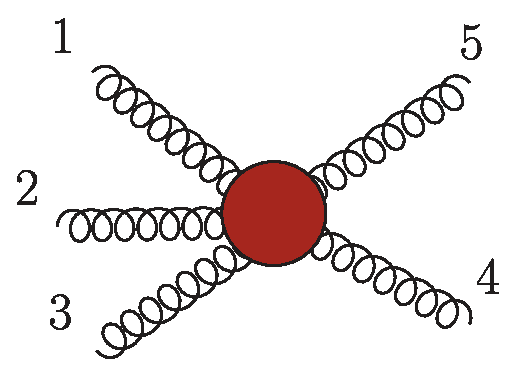
\includegraphics[height=\figureheight]{TreeFull}}} 
    \qquad \xrightarrow[p^2_\xi \to m_\xi^2]{} \quad
    \frac{1}{p^2_\xi - m_\xi^2} \cdot
    \sum_{i\in \text{states}}^{} ~
    \vcenter{\hbox{\includegraphics[height=0.9\figureheight]{TreeLeft}}}\cdot
    \vcenter{\hbox{\includegraphics[height=0.9\figureheight]{TreeRight}}}
  \end{equation*}
  \caption{
    An example of factorization due to a physical pole singularity. 
    Here $p_\xi =  p_1 + p_2 + p_3$.
  }
  \label{fig:factorization}
\end{figure}


\todo{Note that in \cref{eq:optical_theorem} there is a phase-space integral present on the right-hand side}

The exact singularity as expected cannot be reached in any physical process.
However if we analytically continue an amplitude to complex external momenta,
it is possible to choose them to hit the pole explicitly
while still satisfying on-shell conditions for external states.


\subsection{On-Shell Recursion}
\label{sec:BCFW}

The universal factorization  property expressed by \cref{eq:factorization_pole} is independent of perturbation theory. 
For tree-level amplitudes however the factorization can be discovered rather straightforwardly by inspection,
although it might be obscured in the expressions found within the standard Feynman-diagrammatic approach.

The factorization of tree amplitudes can be converted into an algorithm to evaluate them.
This is done through the systematic exploration of the amplitude's factorization limits such that
it can be broken down recursively to sums of lower-multiplicity tree amplitudes. 
The building blocks of this recursion are thus on-shell amplitudes.
This idea is known as \emph{Britto-Cachazo-Feng-Witten} (BCFW) recursion \cite{Britto2005c,Britto2005f}.
The on-shell recursion is a very powerful tool for analytical computations, especially 
in theories with supersymmetry \cite{Dixon:2010ik,Drummond:2008cr,Bourjaily:2010wh}.
However for numerical applications and general models the on-shell recursion algorithm
does not offer benefits over off-shell alternatives, both in speed and numerical stability \cite{Duhr:2006iq,Drummond:2008cr,Badger:2012uz},
especially if one is interested in tree amplitudes in arbitrary number of space-time dimensions (see \cref{chap:numunitarity}). 


\subsection{Generalized Cuts}

Unitarity can be turned into a computational method of loop amplitudes as well.
A certain class of one-loop amplitudes, which
can be written as a sum of box, triangle, and bubble scalar integrals,
\begin{equation} \label{eq:cut_constructable_ampl}
  A^{(1)} = \sum_i d_{i}\,\vcenter{\hbox{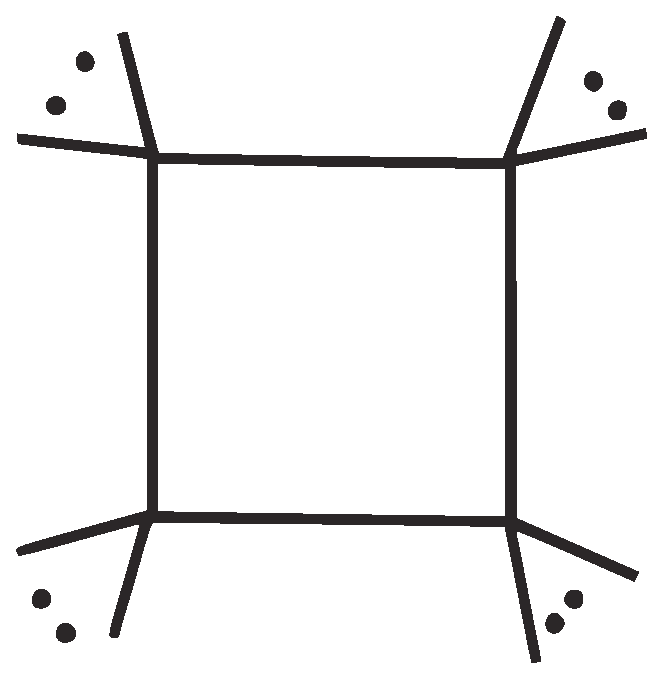
\includegraphics[width=8ex]{boxintegral}}}_i~+~
  \sum_{i}^{} c_{i}\,\vcenter{\hbox{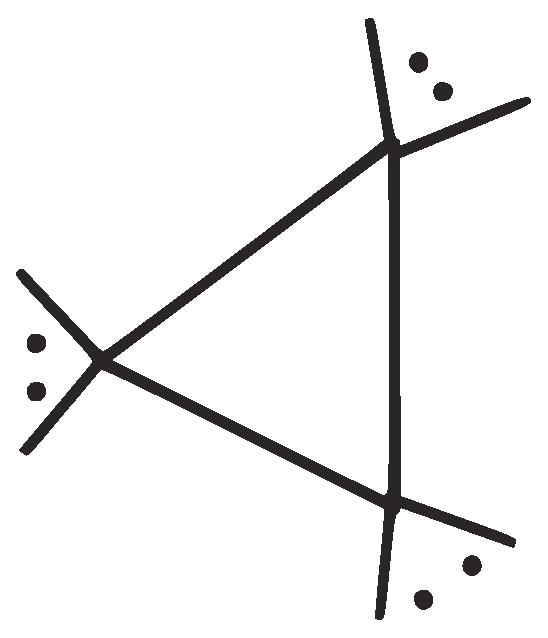
\includegraphics[width=7ex]{triangleint}}}_i~+~
  \sum_i b_{i}\,\vcenter{\hbox{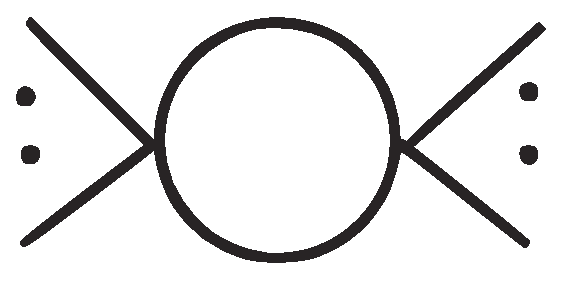
\includegraphics[width=8ex]{bubint}}}_i
\end{equation}
can be obtained entirely from unitarity cuts computed through Cutkosky rules \cite{Bern:1994cg,Bern:1994zx}.
Each integral in \cref{eq:cut_constructable_ampl} has unique discontinuities.
So the discontinuities of the loop amplitude on the left, 
evaluated as phase-space integrals over products of on-shell tree amplitudes as follows from unitarity,
can be matched to those of integrals to obtain equations for the integral coefficients.

However in general \emph{only} unitarity is not enough.

It is possible to generalize application of cuts given by \cref{eq:cut} to
obtain multi-channel discontinuities \cite{Britto:2004nc}.
For example see \cref{fig:quad_cut}.
Note that this kind of cuts are not direct consequences of unitarity of the $\mathcal{S}$-matrix (\cref{eq:unitarity_smatrix}), hence the name \emph{generalized} cuts.

\begin{figure}[ht]
  \centering
  \begin{equation*}
    \vcenter{\hbox{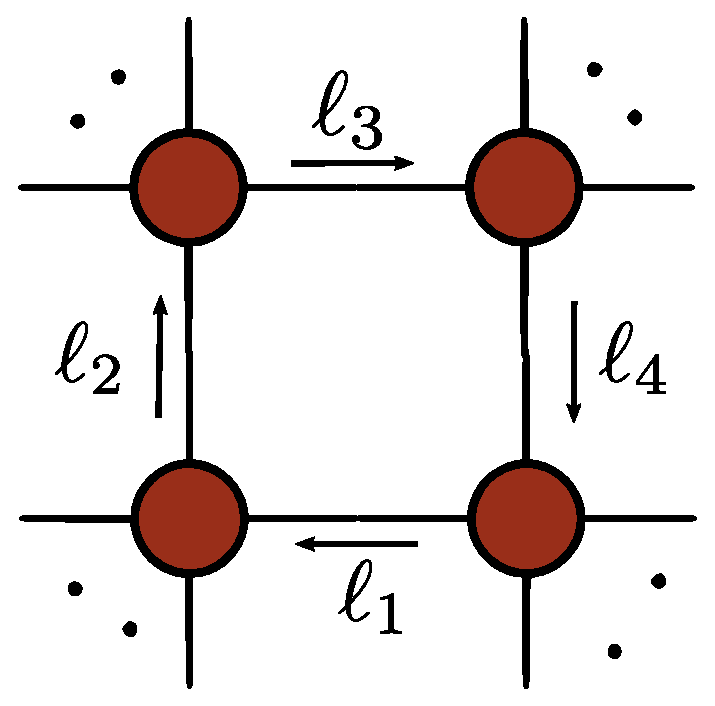
\includegraphics[width=0.2\linewidth]{box}}} \qquad \xrightarrow[i\in\{1\ldots4\}]{\ell_{i}^2-m_i^2\to~0} \qquad
    \vcenter{\hbox{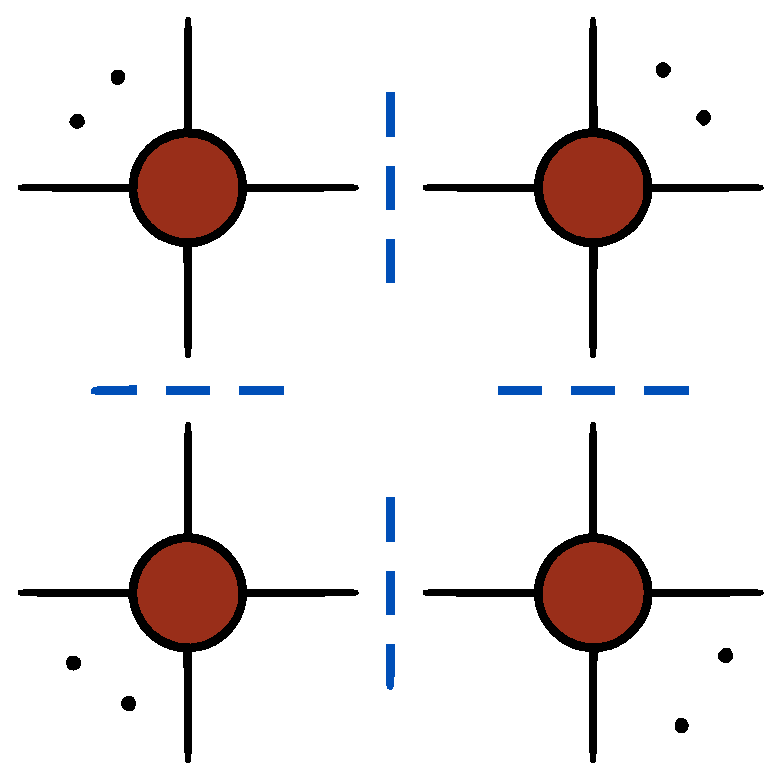
\includegraphics[width=0.2\linewidth]{boxCut}}}
    \quad = \quad \sum_{i}  c_{i} ~ m_{i}(\ell) %+ \sum_{i}  \tilde{c}_{i} \,\tilde{m}_{i}(\ell)
  \end{equation*}
  \caption{
    An example of a generalized cut.
    The loop momentum is chosen such that four propagator are simultaneously put to zero.
    On the left \emph{all} diagrams with the chosen propagators contribute.
    In the factorization limit each corner is a tree amplitude.
    The cut is matched to a basis of loop-momentum polynomials $\{m_i(\ell)\}$ on the right.
  }
  \label{fig:quad_cut}
\end{figure}


As a next step one can use the factorization of amplitudes on the cuts at the \emph{integrand} level  and match
it to a basis of loop-momentum polynomials in numerators (see \cref{fig:quad_cut}),
instead of integral coefficients \cite{Giele:2008ve,Ellis:2007br,Ellis:2008ir,Berger:2008sj}.
This matching procedure is intimately connected to a purely algebraical method of integral reduction known as OPP \cite{Ossola:2006us}.
This method uses the cut conditions \cref{eq:cut} to set some propagators to zero and triangularize linear systems for determining the basis coefficients.
It can be applied individually to each Feynman diagram or a sum thereof, thus having very little to do with factorization and unitarity.
When applied to the full amplitude however, it re

\todo{here unfinished} 
Somewhat confusingly sometimes generalized unitarity methods also refer 

Its flexibility allows for straightforward automation (see e.g.\ \cite{Berger:2008ag,Berger:2008sj,Cullen:2011ac,Mastrolia:2010nb,Ossola:2007ax}).

Most of the ideas mentioned in this section are formulated in the context of one-loop computations.
These give the first real taste of quantum nature of QFT.
Unfortunately, going beyond one-loop, many of the ideas do not generalize straightforwardly,
and require much more sophisticated computational techniques.
The extension of the ideas to multi-loop level have been actively studied in recent years \cite{Ita:2015tya,Abreu:2017idw,Abreu:2017hqn} 

In this thesis we apply the state-of-the-art developments for 

